\section{The archive} 

At the time of writing, the full ULTRACAM archive is still undergoing analysis by the automated pipeline. At present \emph{159} nights, out of a total of \emph{390}, have been processed and are available for viewing at the following URL: \url{http://url.to.be.provided/}. Of these processed nights, approximately \emph{xx} have been investigated for variability. At the moment, the investigation is almost purely visual, based on a human inspecting each light curve. The web interface is designed so that it is easy for the viewer to examine the light-curves of all of the objects systematically. The user-interface allows the users to see each light curve, one-by-one by press the 'right' and ;left'  arrow keys on the keyboard. More information on how to use this interface can be found in the User Manual~\ref{chap:usermanual}. 

\section{Data quality}

\subsection{Photometric calibration}
The main purpose of this MSc project was to establish a process for automatically reducing the light-curves for all objects in the data archive rather than to focus on accurate and well-calibrated measurments. The diverse nature of the dataset means that it is not trivial to write a purely automated algorithm that can perform fully calibrated measurements. 

Correct calibration of the photometry for ULTRACAM requires to the following steps:
\begin{itemize}
  \item Using \emph{flat fields} to take into account the varying sensitivity of the CCD detector across the field. 
  \item Subtracting \emph{bias} frames from each image to remove the additional counts caused by having a non-zero bias on the CCD. 
  \item Using a \emph{standard star} to produce offset brightness to calibrate to the standard magnitude system. For ULTRACAM these are usually Sloan u, g, r, i magnitudes.
  \item Computing the \emph{atmospheric extinction} for the night by fitting extinction curves for a number of bright objects that have been measured over a range of airmass. 
\end{itemize}
During a typical night at the telescope, the observer will take steps to ensure that there is sufficient data to perform this calibration. They will take several bias frames, flat-fields and will observe standard stars. When the reduction is performed later, these various datasets will be combined to calibrate the photometry of the target objects. 

The automated pipeline built for this project lacks the ability to correctly identify the correct bias reading, flat-fields and standard stars that should be used for photometric calibration. This would require human intervention. Therefore, this step is skipped altogether. The magnitudes and flux counts produced by the pipeline are \emph{not} calibrated and will differ from their true values by a certain offset.

It is possible to take the output of the automated pipeline and calibrate the photometry, but, at the moment, this is a manual process. 

\subsection{Comparison of the 2 pipelines}
Since the ULTRACAM already has a well-established data reduction pipeline, it is useful to compare the results of this pipeline with the new, automated one built in this project. As mentioned above, the automated pipeline does not perform calibrated photometry, but we can still compare the non-calibrated photometry to get an estimate of how well our new pipeline performs.

In order to do this, we chose a run of a target object that has often been observed with the ULTRACAM. The object is \emph{NN Ser}, a white-dwarf, M-dwarf eclipsing binary. The specific run in question is \emph{2013-07-13/run111}.

Running the automated pipeline on this run is acheived simply by typing: \begin{verbatim}runbuilder.py 2013-07-13/run111 \end{verbatim} on the command line. Please refer to the user manual \cite{chap:usermanual} for instructions on how to install and run the pipeline.  The reduction takes about 5 minutes of processing time running a standard desktop machine in the University of Warwick Astronomy department. The output of this reduction can be seen at \url{http://deneb.astro.warwick.ac.uk/phrnaw/sitedev/2013-07-13/run111.html}.

\begin{figure}[!h]
\centering
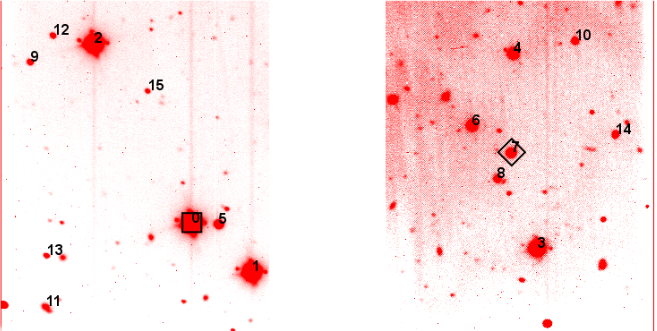
\includegraphics[width=120mm]{images/2013-07-13-run111-r-withlabels.png}
\caption{Snapshot taken from the automated pipeline browser for 2013-07-13/run111, target:NNSer. This is a stacked image from the 'red' CCD with the Sloan 'i' filter. }
\label{fig:nnserfield}
\end{figure}

\begin{figure}[!h]
\centering
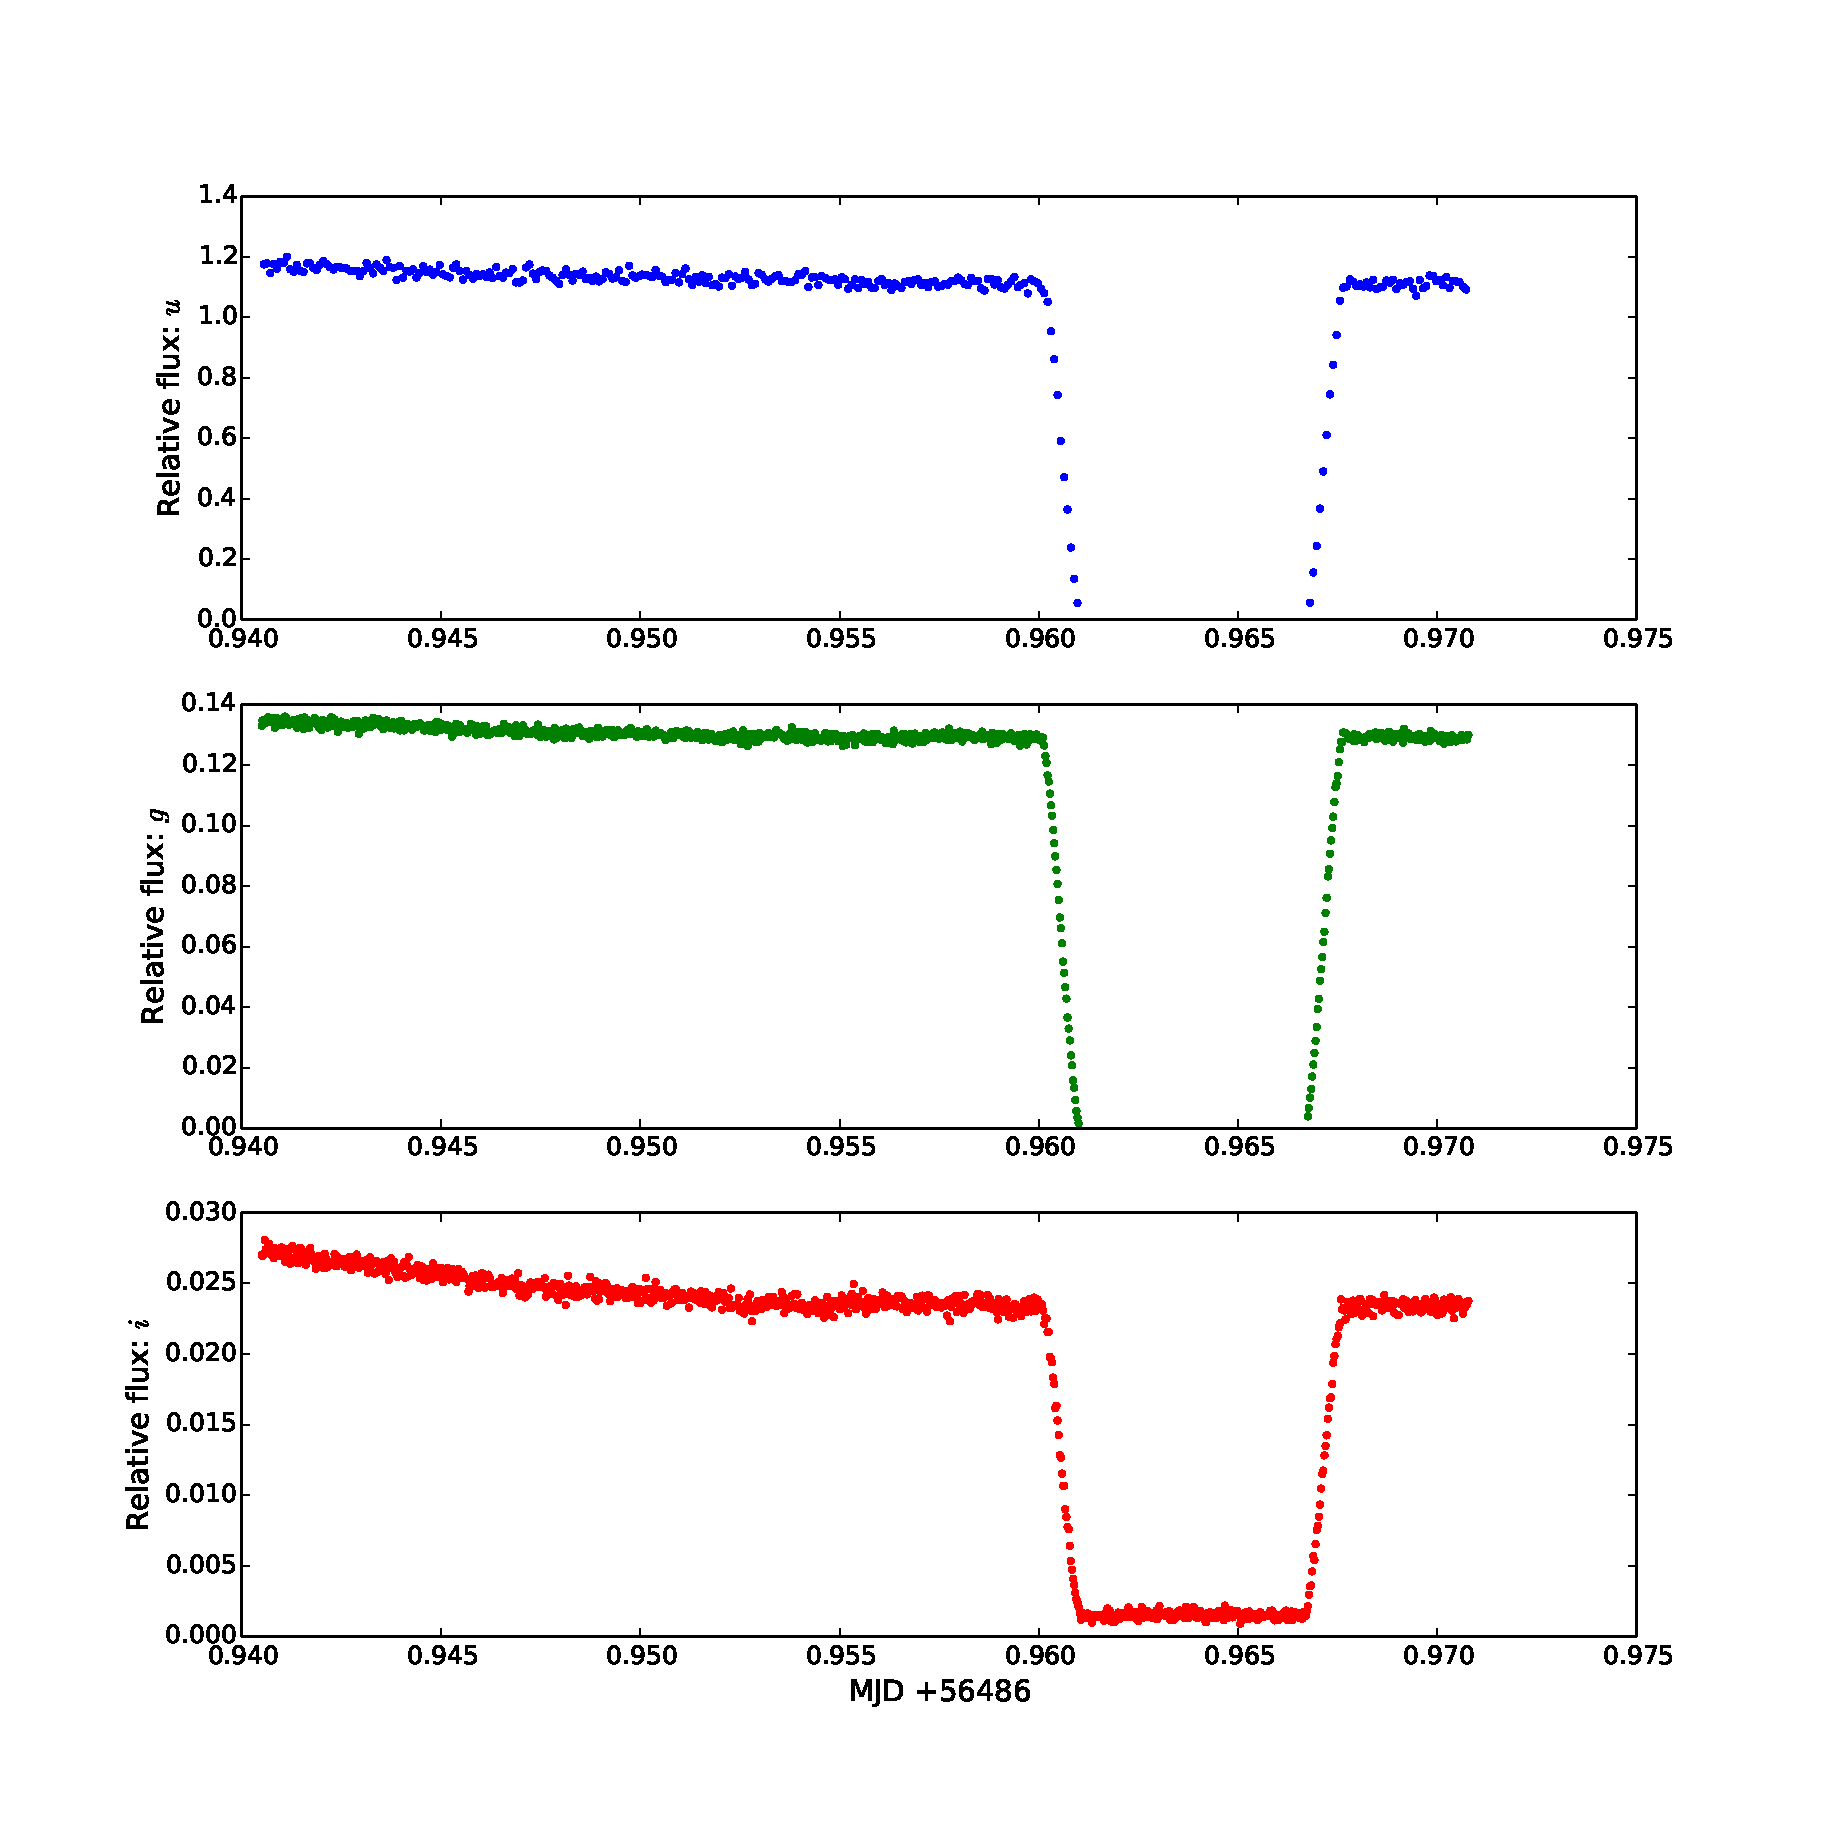
\includegraphics[width=140mm]{images/nnser_lightcurve_automated.eps}
\caption{Light curve of the target object, NN Ser produced using the \emph{automated pipeline}. The vertical axis is the raw flux measurements calculated by SExtractor.}
\label{fig:nnserlightcurveautomated}
\end{figure}

\begin{figure}[!h]
\centering
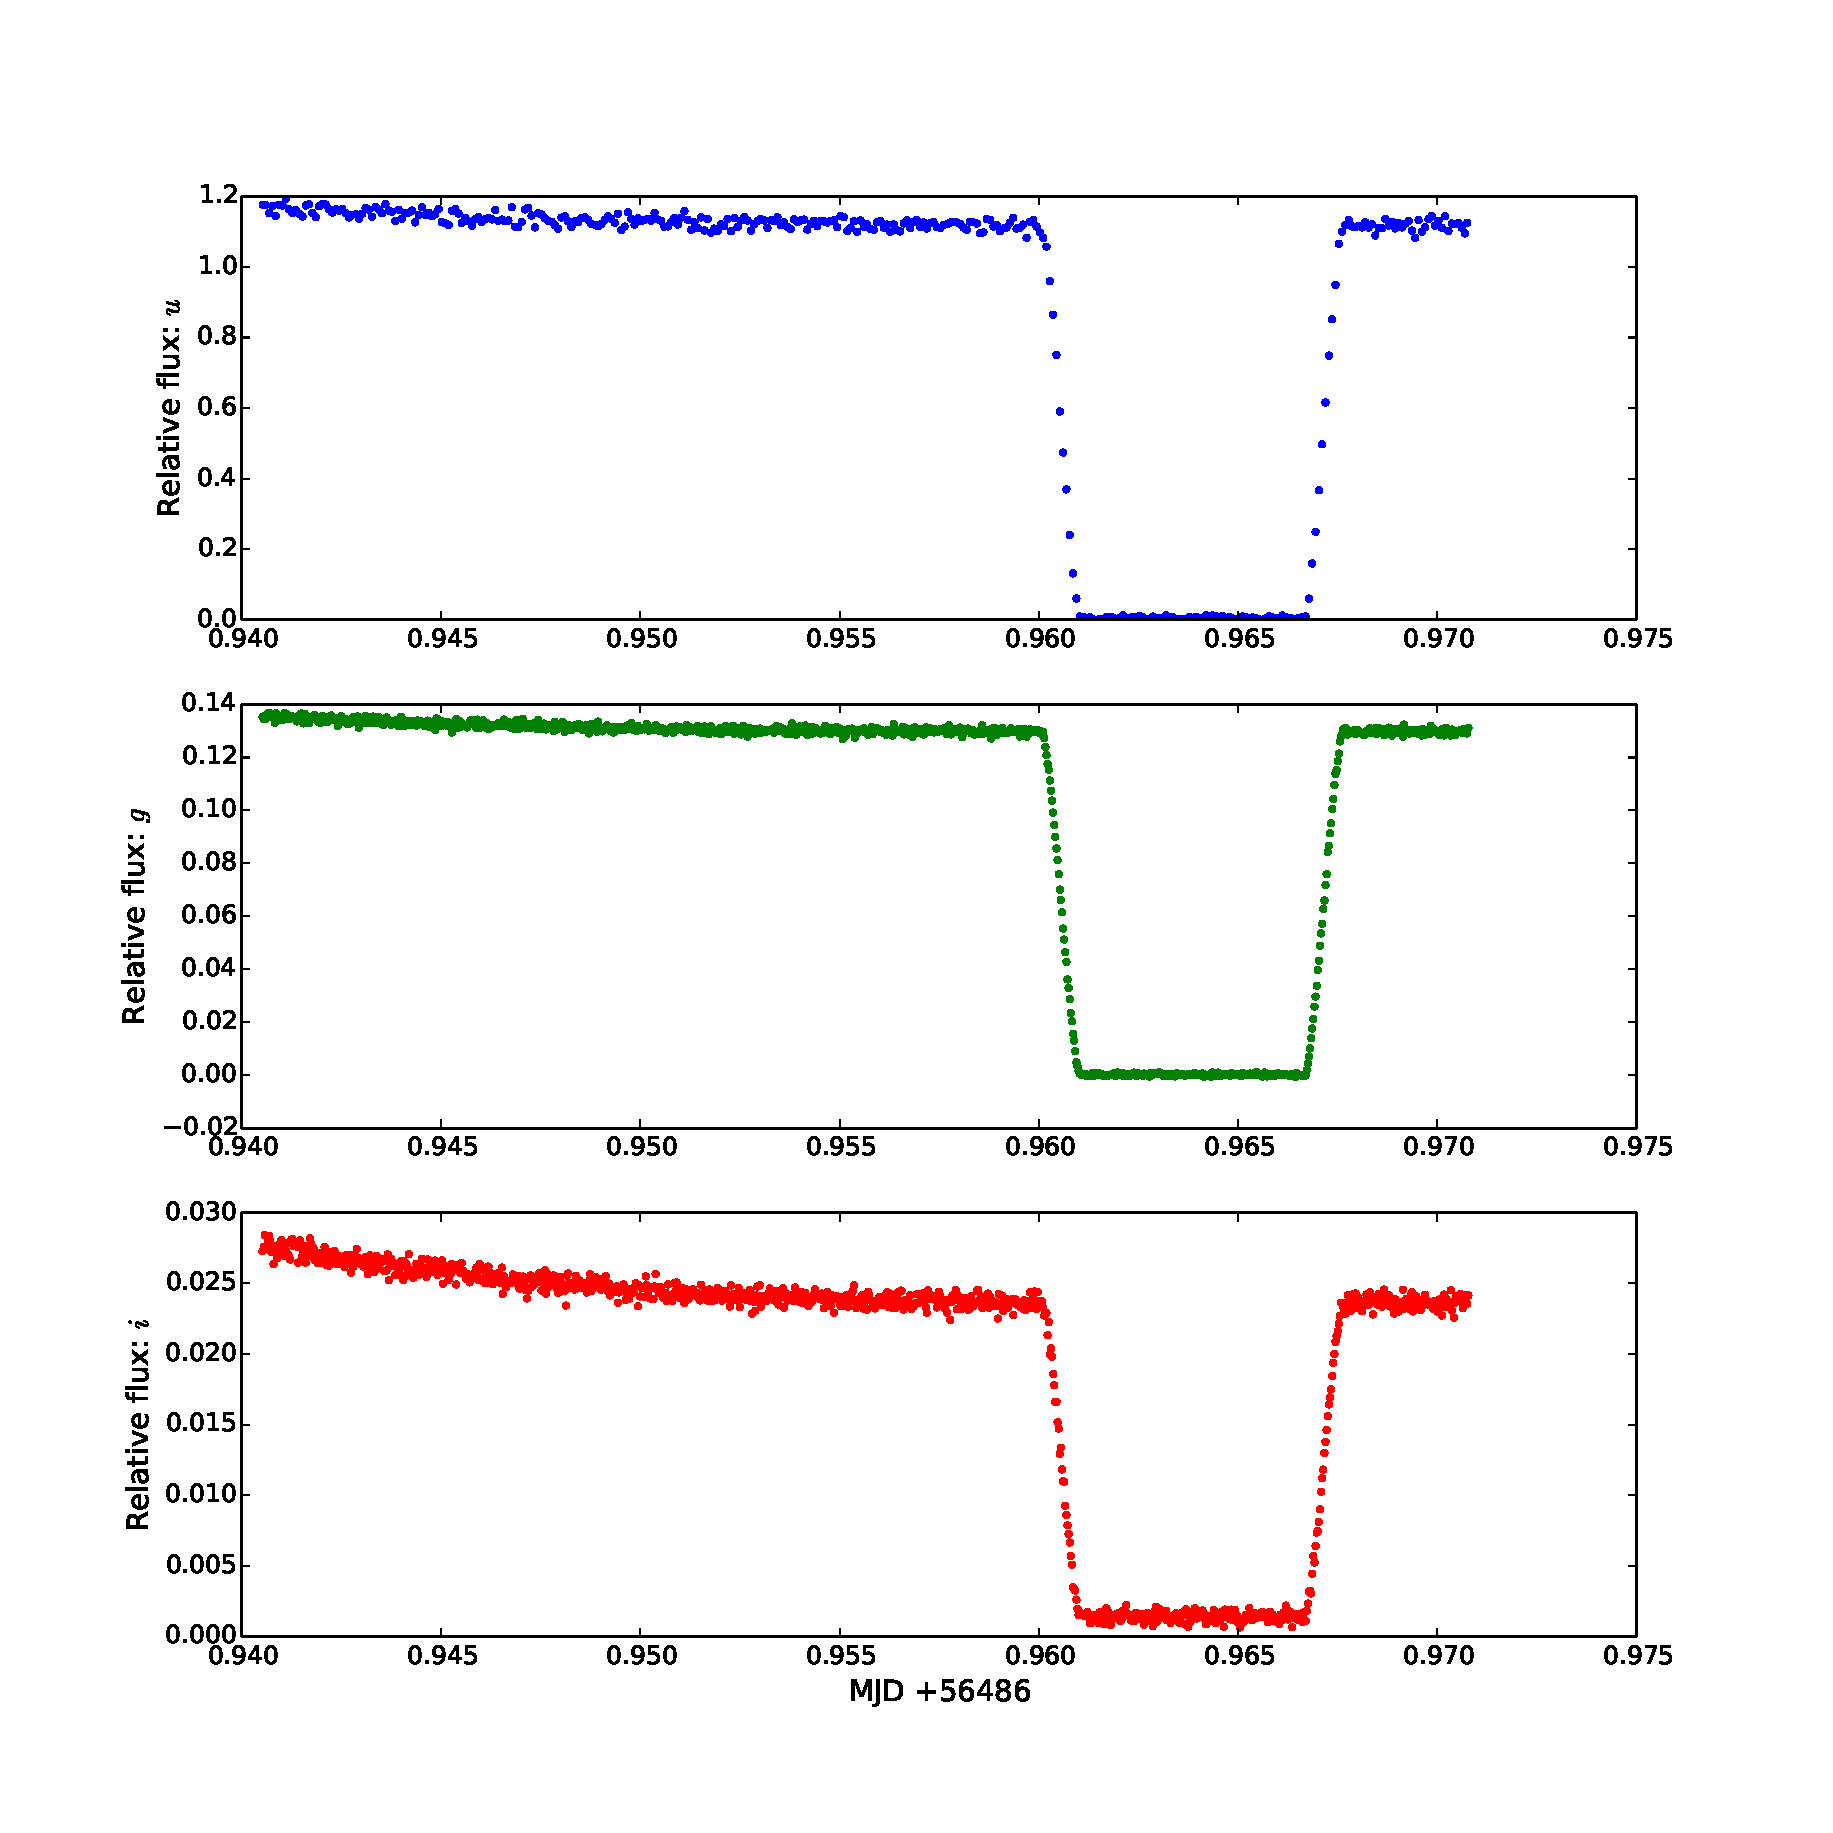
\includegraphics[width=140mm]{images/nnser_lightcurve_tom.eps}
\caption{Light curve of the target object, NN Ser, produced using the \emph{standard pipeline}. Comment: Does Tom's pipeline automatically remove sky counts?}
\label{fig:nnserlightcurvetom}
\end{figure}


\begin{figure}[!h]
\centering
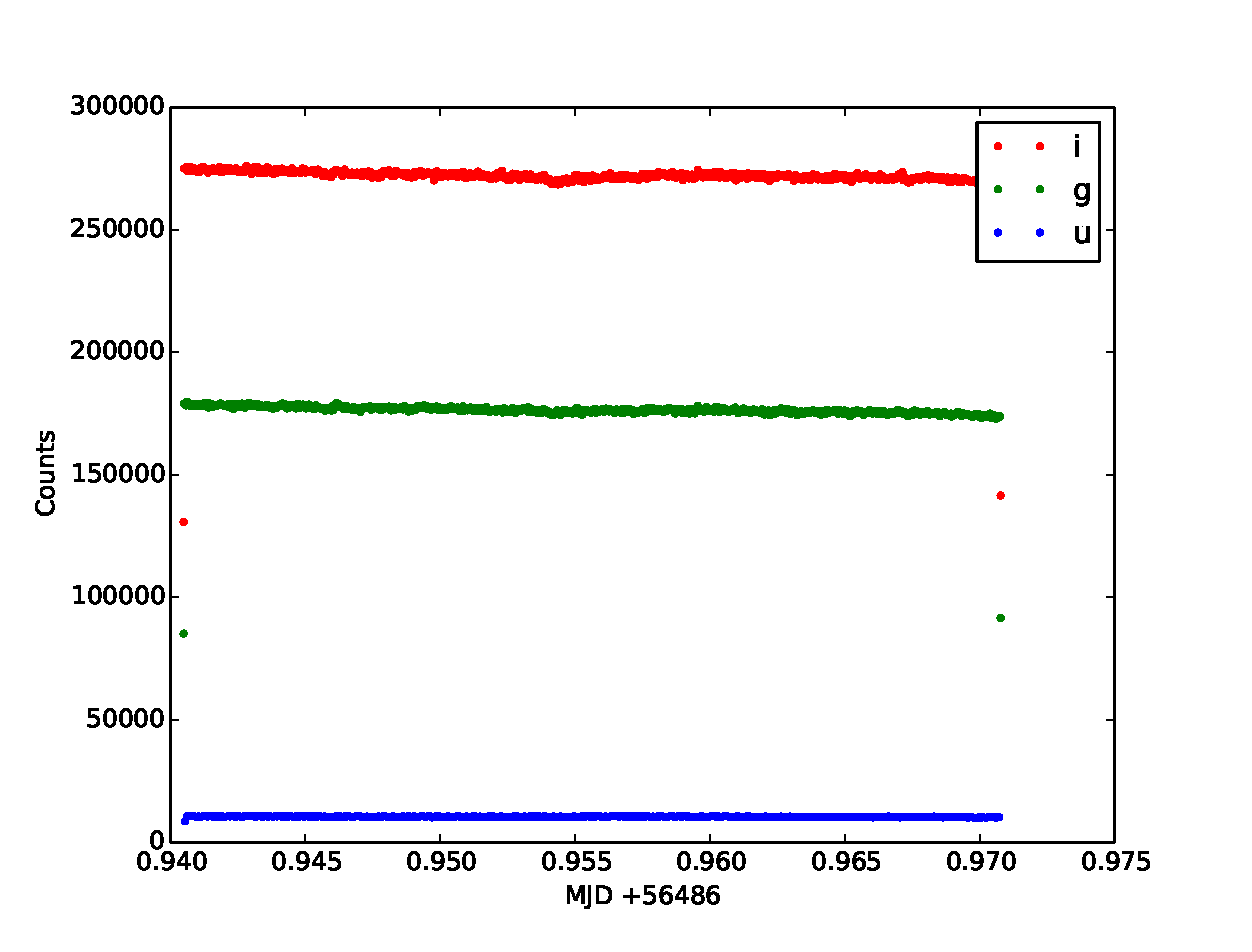
\includegraphics[width=140mm]{images/comparison_auto.eps}
\caption{Light curve of the comparison object, labeled '0' in figure \ref{fig:nnserfield}. This lightcurve was produced by the \emph{automated pipeline}. The vertical axis is the raw flux measurements calculated by SExtractor.  }
\label{fig:nnsercomparisonauto}
\end{figure}

\begin{figure}[!h]
\centering
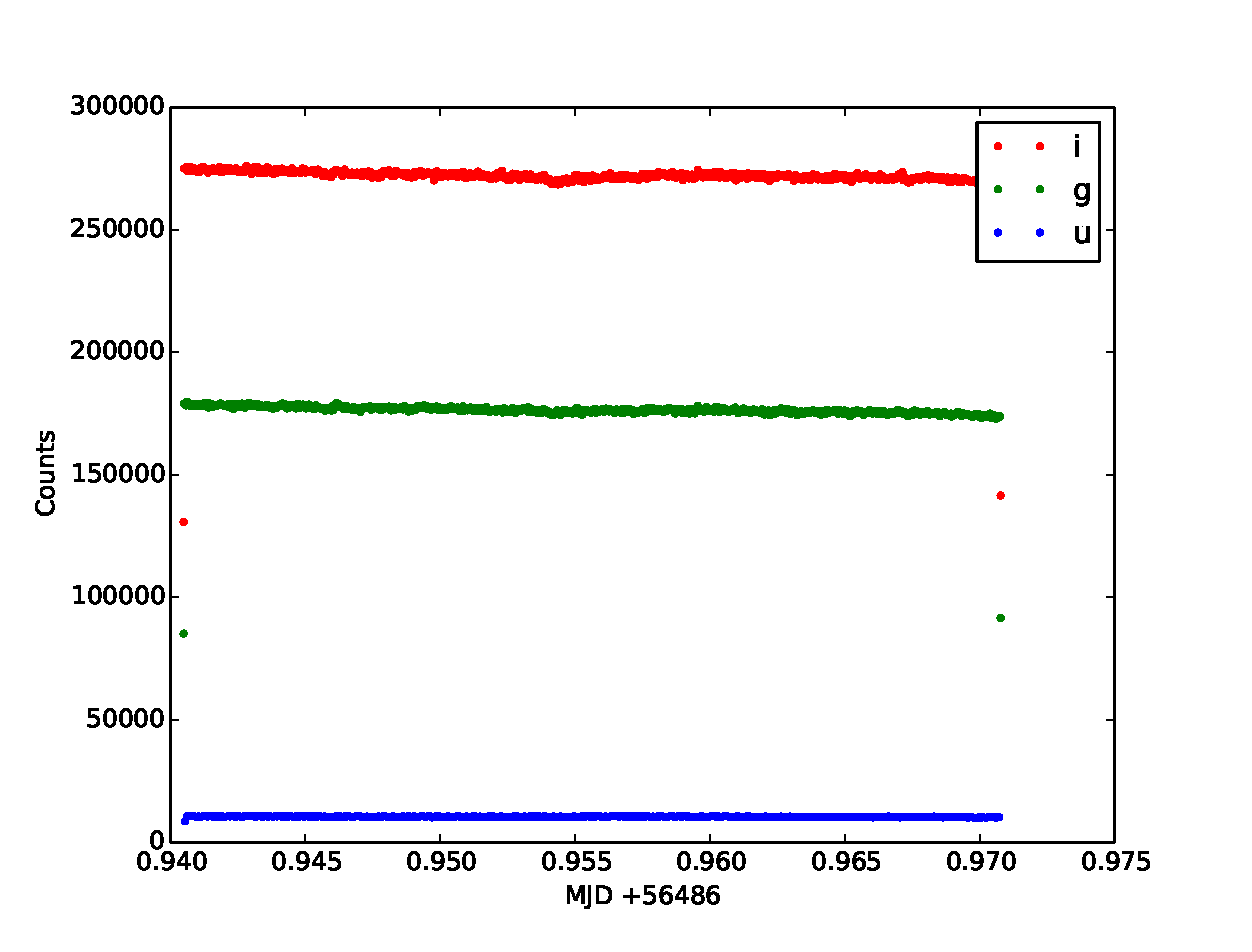
\includegraphics[width=140mm]{images/comparison_auto.eps}
\caption{Light curve of the comparison object, labeled '0' in figure \ref{fig:nnserfield}. This lightcurve was produced by the \emph{traditional pipeline}. }
\label{fig:nnsercomparisontom}
\end{figure}

To reduce the same run using the standard pipeline, we defined apertures for the objects we wanted light curves for. In this case, we are interested in the objects labeled \emph{7} (the target 'NN Ser') and \emph{0} (a comparison star) in figure \ref{fig:nnserfield}. We set up the apertures manually using the \emph{setaper} tool. 

\subsection{Residuals}
The plot in figure \ref{fig:residualplot} shows the residuals of the photometry created by subtracting the flux counts measured by the automated pipeline from those measured by the traditional pipeline. There is a systematic offset for each channel which suggests that the automated pipeline overestimates the flux by xx percent. This is due to.... 

\begin{center}
	\begin{tabular}{|l|r|r|}
		\hline
		Filter & Mean counts & Standard deviation\\
		\hline
		'i' & 272138 & 4372 \\
		'g' & 590943 & 494 \\
		'u' & 404044 & 4878\\
		\hline
	\end{tabular}
\end{center}


\begin{figure}[!h]
\centering
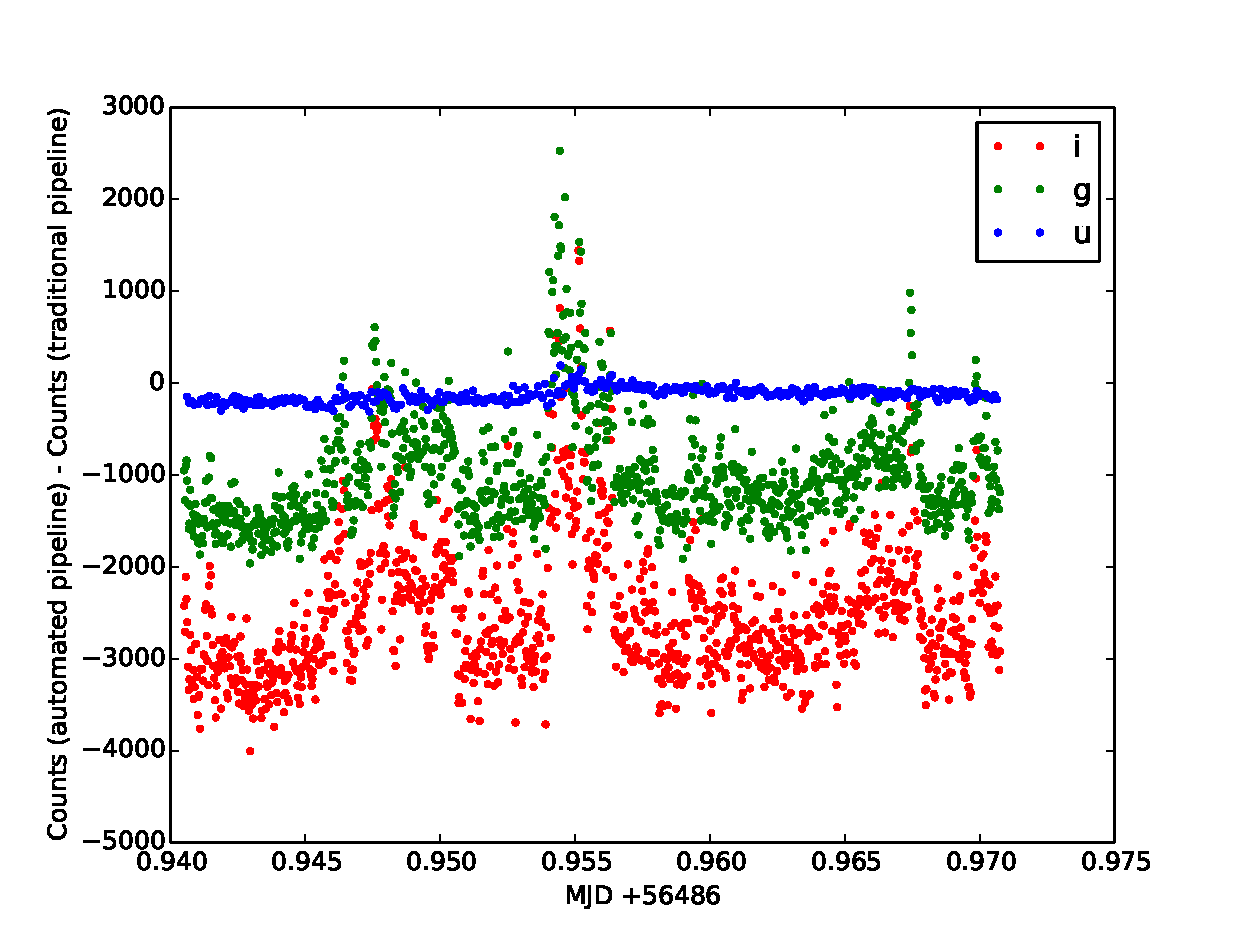
\includegraphics[width=140mm]{images/residuals.eps}
\caption{A plot of the residuals created by subtracting the flux counts derived from the \emph{traditional pipeline} from those derived using the \emph{automated pipeline}. }
\label{fig:residualplot}
\end{figure}

\subsection{Apertures}
Since the automated pipeline relies on the third party software, SExtractor, to determine the apertures on each frame, objects that do not meet the required signal to noise ratio on any particular frame will not be detected and therefore have no aperture defined for that frame. This means that objects that fade or are generally quite faint, might 'disappear' on some frames and then 're-appear' on subsequent frames. The tracking algorithm allows a 're-appearing' object to be identified with an object that appeared on previous frames provided that the pixel location is roughly similar. An illustration of this can be seen in figures \ref{fig:nnserlightcurveautomated} and \ref{fig:nnserlightcurvetom} where the automated pipeline 'loses' the target object in the 'g' and 'u' bands after the ingress of the primary eclipse, but picks it up again at the start of egress. In contrast, the traditional reduction pipeline can have apertures that are linked to other objects in the field and can therefore continue to calculate flux in the aperture for the target even if the target is barely detectable above the sky background.


\section{Highlights}

Some 'interesting' objects discovered by the pipeline.


